%!TEX root = foo-thesis.tex


\chapter{Implementation}
\label{chap:implementation}

\todo{mention repository. decide on repository name, and maybe github name. give the repository a license.}

\section{Used Framework and Libraries}

\begin{figure}[htbp]
  \centering
  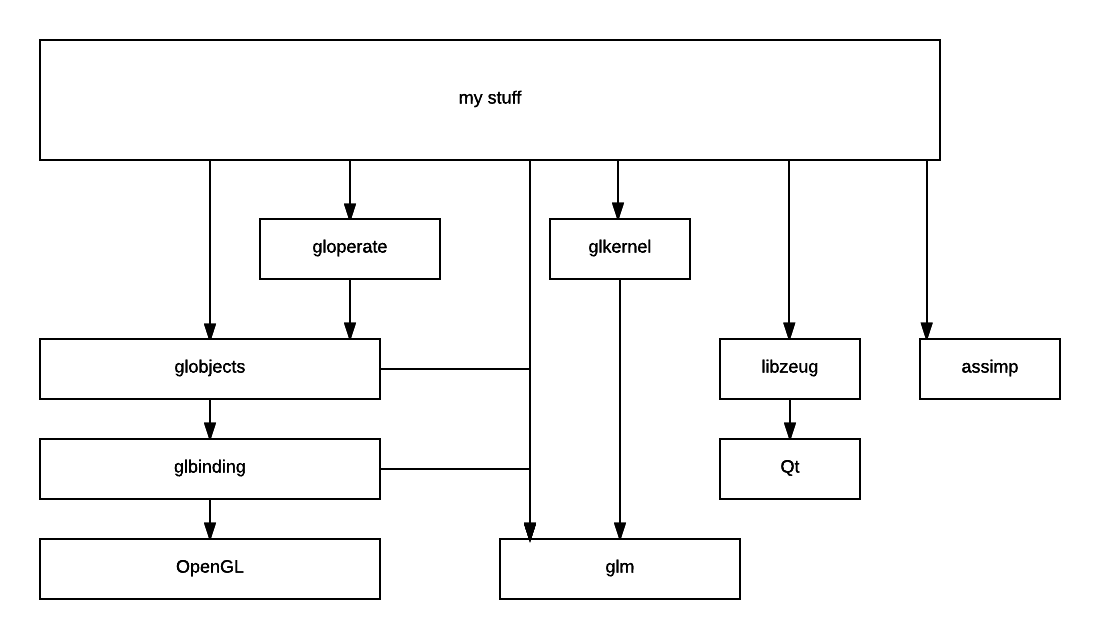
\includegraphics{graphics/Architecture}
  \caption{svg image}
\end{figure}

The implementation was built using C++ and OpenGL. It uses \textit{gloperate}\footnote{\url{https://github.com/cginternals/gloperate}} as framework, which provides some basic functionality like navigation and resource handling. \textit{gloperate} in turn is based on Qt\footnote{\url{https://www.qt.io/}}, which is used for context creation and the UI. \textit{libzeug}\footnote{\url{https://github.com/cginternals/libzeug}} is used to provide GUI widgets for quick manipulation of the rendering's parameters.

\textit{globjects}\footnote{\url{https://github.com/cginternals/globjects}} provides a convenience abstraction layer around the OpenGL API, which is in some places directly accessed using \textit{glbinding}\footnote{\url{https://github.com/cginternals/glbinding}}. For math functions and interaction with \textit{globjects}, \textit{glm}\footnote{\url{http://glm.g-truc.net}} is used.

Additionally, \textit{assimp}\footnote{\url{http://www.assimp.org/}} is used to load the test scenes.


\section{Rendering Pipeline Overview}
\begin{outline}
\1 would be much the same as the concept pipeline...
\1 show what's compute shader and what not?
\1 it's basically lighting plus
    \2 g-buffer generation
    \2 shadow map which is part of the RSM,
    \2 SSAO
    \2 deferredshading
    \2 srgb and HDR.
    \2 all of this is not
\1 model loading?
\1 kernel generation?
\end{outline}

\todo[color=blue]{textify rendering pipeline overview implementation}


\section{RSM Generation and VPL Sampling}
\label{sec:impl:rsmAndVplSampling}

The RSM generation mostly uses the same code as the G-Buffer generation, barring a few modifications: First, normal maps are ignored and triangle normals are used instead, and instead of individual texture lookups during shading, the material's average color is used as diffuse color. Both these changes are made in order to avoid high-frequency normal and changes in the RSM, which can only be captured correctly with a larger number of VPLs.

Additionally, the RSM is re-used as conventional shadow map. Usually, one might want to decouple RSM and conventional shadow map generation to use different resolutions or cascading schemes. It would also be possible to render the RSM with a less detailed version of the scene. Since we had no culling and LOD techniques available, we were bottlenecked on geometry complexity and chose to render both RSM and conventional shadow map in one pass. As a result, we render one additional variance buffer for use with the variance shadow mapping technique \citep{Donnelly:2006:VSM}.

Following the RSM generation, a compute shader samples the RSM in a regular pattern and writes the world-space position, normal and color of the sample points into a separate buffer. These information form the VPLs.

Additionally, a second buffer is prepared that, instead of three three-component vectors, stores only one four-component vector, holding the VPL's position in the first three components and the normal packed into the last component. This is done since the ISM rendering (\Cref{sec:impl:ismRendering}) and light list calculation (\Cref{sec:impl:clusteredShading}) do not need the color information and especially the ISM rendering reads several VPLs per point, using a lot of bandwidth.


\section{ISM Rendering}
\label{sec:impl:ismRendering}

Both the point splat renderer and the single-pixel point renderer share the first stages of their rendering pipelines, which are described here, before the following subsections describe the two renderers themselves and the pull-push postprocessing.

We make use of OpenGL's tessellation shader to subdivide triangles to make them meet a certain maximum size. The tessellation control shader determines the tessellation levels according to the triangle's size. The tessellation evaluation shader does nothing more than correctly interpolating the vertex positions.

The geometry shader, which now recieves the smaller, tessellated triangles, converts each triangle to a point. The point's center equals the triangle's center, and the radius is chosen so the areas of the point and triangle match.

\todo[color=yellow]{implement that area thing}

While a random subset of all points needs to be chosen for each ISM, special care must be taken to make sure that the same subset of points is used for each ISM in each frame. Otherwise, the ISMs will be temporally incoherent and cause flickering in the final rendering. To this end, the point's barycentric coordinate inside its triangle and the triangle's \texttt{gl\_PrimitiveID} are passed to a fast hashing algorithm. The result is is used to determine an ISM ID (or, equivalently, a VPL ID) for use in the next step.

Note that no translation or projection has been applied yet, this happens in a later stage. As a result, the vertex shader is a simple pass-through shader.

The next step depends on whether point splatting or the single-pixel renderer is enabled.



\subsection{Point Rendering with Splatting}
\label{sec:impl:splatting}

In the case of point splatting, the geometry shader itself reads the VPL with the ID it determined, projects the point according to the VPL's data, performs culling and discards the point if necessary, sets \texttt{gl\_PointSize} to the projected size, and emits a vertex.

The \texttt{output\_primitive} must be set to \texttt{points} in the geometry shader's \texttt{layout} definition. As explained previously, for point splatting all points are simply enlarged by a small constant factor in lieu of the pull-push postprocessing. Since only depth information are needed in this case, the fragment shader is empty.



\subsection{Single-Pixel Point Rendering with Compute Shaders}
\label{sec:impl:singlePixelRendering}

This approach was inspired by the fact that the surface reconstruction in \citet{Marroquim:2007:reconstruction} works with single-pixel ``splats''. Since in this case the hardware rasterizer is not required to achieve good performance, this allowed for more flexibility and new optimization opportunities.

The general idea is to first let the geometry shader write the generated points into a buffer, which is then used by a separate compute shader pass to perform the actual rendering.

In order to maintain temporal coherence, the points are not written into a single large buffer, as it would be hard to consistently determine a location for each point in that buffer. Instead, the buffer is divided into one section per VPL, and the points are written into the section corresponding to the ID calculated before. An atomic counter that indicates the first free index is used per section to sequentially fill these sections without overwriting any data. The order of the points within each section is undefined, but that does not change the output since they all are going to be rendered into the same ISM.

Now a compute shader is used to render the points. For each VPL, one work group reads through the respective section of the point buffer and performs the transformation and culling against the VPL for each point. It then uses \texttt{imageAtomicMin} to ``render'' the point with correct depth testing as a single pixel into the respective ISM. Since atomic operations require using single channel integer textures, it is not possible to use a second or third channel for additional attributes. Instead, one 32\,bit channel is used, with 24\,bits containing the depth, and 8\,bits containing the radius, which is the only attribute that is saved. Since the depth is in the 24 more significant bits, the depth test still works correctly. Another version that used a 3D texture for additionally storing the normal was implemented as well, see the next subsection.

As an optimization, the compute shader renders each point into several ISMs. To this end, each work group reads the data of a fixed number of VPLs (e.\,g.\ 16) into shared memory. Then, while rendering the points, the culling is performed per point on all 16 VPLs, and those VPLs where the point passes the culling test are collected into a local array. Thereafter the point is transformed for each of the collected VPLs and rendered into the respective ISM.

% In practice it turned out to be more efficient to limit the number of slots in the local array to a constant maximum (e.\,g.\ 4), possibly because this ensures that the rendering loop is not diverging and enables compiler optimizations like loop unrolling.

An attempt to do this optimization in the splat renderer by emitting multiple vertices in the geometry shader resulted in a significant performance hit, see \Cref{sec:results:ism:performance}.


\subsubsection{Issues when storing normals}
\label{sec:impl:raceCondition}

For a higher-quality postprocessing, the normals of the points are required. Since we did not use the normals in our final version, we were able to follow the simplified one-channel approach described above, but we had implemented a different version that also stored normals. The issues we faced when implementing it are described here.

Instead of using a one-channel 2D texture for the ISM, where the single channel contained both the depth and radius, a 3D texture where the third dimension has a depth of two can be used. The first index of the third dimension would hold the depth, while the second index is used as additional ``render target'' to hold the radius and normal.

Besides roughly doubling the time needed to render the points due to the increased bandwidth, this implementation introduces a second race condition besides the usual z-fighting that can occur.

First, the order of writes to the ISM depth buffer is undefined as the execution order of the different compute shaders is undefined in the OpenGL specification. Therefore, the classical z-fighting may occur if two points are rendered into the same pixel of the same shadow map with the same depth value. The attributes that end up written into the additional render target are undefined in this case and may differ between subsequent frames. In practice, this happens very rarely and we chose to ignore this.

However, a different race condition was frequently observable in our implementation:
If two threads with differing depth values simultaneously write into the depth buffer, using \texttt{imageAtomicMin} guarantees the correct value will end up in the buffer. However, if the higher value got written first and gets overwritten by the second write, both writes have succeeded. This results in both threads attempting to write into the second buffer, creating another race condition since the here execution order is undefined again. This problem can be alleviated by adding a synchronization point after the atomic write and then reading the memory location that just got written to. If it is equal to the written value, one can assume the write actually succeeded and did not get overwritten by a second, simultaneous write. Only then the write to the second buffer is performed.

This solution had little cost (0.08\,ms), but fixes the race condition only inside one work group and not between work groups, for which no efficient synchronization primitives exist on the GPU. On a NVIDIA GTX 750 Ti, the race condition was still observable but not annoying. Interestingly, on a GTX 980, the race condition seemed to not occur at all with the described workaround.

A proper solution that would fix this problem completely, avoid the synchronization overhead and open more optimization possibilities would involve a more advanced software renderer, e.\,g.\ following the approaches of \citet{Laine:2011:SoftwareRasterization}.


\subsection{Pull-Push Postprocessing}
\label{sec:impl:pullPushPostprocessing}

Our implementation of the pull-push algorithm is relatively straightforward. For each miplevel to be calculated, one \texttt{dispatchCompute} is called. Since the first step of the pull phase has different inputs than the subsequent steps (it only has depth and size, not the displacement vector and depth interval), a slightly different shader is used there. Analogous the last step of the push phase outputs only depth, therefore a shader variant is used for that step as well. For the same reason, the input texture (the ``render target'' used by the single-pixel renderer) and output texture (the final ISM used later for shadowing) have different formats than the mipmap levels used by the pull-push algorithm.



In the pull phase, one compute shader invocation calculates one output pixel. It reads its four input pixels, determines which of them are valid, and uses the valid ones for interpolating.


During the push phase, groups of four output pixels share the same input pixels. This can be exploited by letting each shader invocation compute four output pixels while still reading only four input pixels. Naturally, the weights applied to the input pixels need to be adjusted per output pixel. For invalidating input pixels, their weights can simply be set to zero instead of separately marking them as invalid.

Note that there is still lots of room for optimization. Especially the pull phase is basically a parallel reduction which is well-researched and for which optimized algorithms on the GPU exist, see e.\,g.\ \citet{Harris:2007:ParallelReduction}. Several optimizations from that field might be applicable here.



\section{Interleaved Shading with Compute Shaders}
\label{sec:impl:interleavedShading}

The presented implementation performs interleaved shading, that is, it processes only a fraction of all VPLs per pixel and uses a blur pass to mask the resulting noise. Since adjacent pixels now process different sets of VPLs, this approach results in low cache coherence. To this end, de-interleaving has been proposed \citep{segovia2006non}.

Often, de-interleaving is implemented by splitting the G-buffer into several smaller G-buffers, each containing all pixels with the same sample set. Each G-buffer is processed with its respective sample set, and then the buffers are re-interleaved into a large G-Buffer again.

We propose to perform de-interleaving, sample processing and re-interleaving in a single pass using compute shaders. Just like with the original method, each work group processes a set of pixels that use the same set of VPLs. But instead of performing coherent reads and writes, making it necessary to first split the G-Buffer and then re-interleave it, we propose to let the compute shader read and write directly to the respective pixels in the G-Buffer. See \Cref{???} for a comparison of the two approaches.

\todo{Figure: interleaved shading: Compare buffer splitting vs compute shaders}

There are several reasons for this approach: First, it is easier to implement, since the buffer splitting and re-interleaving phases are not needed anymore. Second, as another consequence of eliminating these phases, the total amount of memory read and written is greatly reduces, potentially saving bandwidth. And third, no additional storage is needed.

A potential downside is that this technique performs one scattered read of the G-Buffers, compared to several coherent reads performed by the buffer splitting method. However, the bottleneck of the final gathering phase lies within the loop over the VPLs, so this one-time scattered read is likely to not have any impact but to be swallowed by latency-covering techniques of the GPU. Theoretically, the works groups could be distributed over the GPU's processor clusters (Streaming Multiprocessors on NVIDIA, Compute Units on AMD) in a way that adjacent pixels are still processed on the same cluster, but unfortunately application developers have no control over this.

\todo[color=yellow]{investigate into interleaving via shared memory in 2x2 groups}
\todo{write hedman, how did they do the 8x8 interleaving? or maybe check his master thesis first}

Since only a subset of all samples is processed per pixel and this subset repeats every four pixels, interleaved shading results in structured noise. (see Figure \ref{fig:???} or this figure in concept?). To this end, a geometry-aware blur similar to \citet{laine2007incremental} is often used. The geometry-awareness is needed to prevent light from bleeding over geometry edges. Although the blur filter is not separable due to its geometry-awareness, we implement it in a separated fashion, trading a neglibile quality impact for large performance benefits.

\todo{implementation: interleaved: figure of noise here? or just in results?}


Because of the regular sampling, the noise produced during interleaved shading (\Cref{sec:impl:interleavedShading}) is more structured and harder to mask by the blur pass. To alleviate that, we permutate the VPL order with a random permutation computed on the CPU. See \Cref{sec:results:interleavedShading} for the effects of this small optimization.

While the geometry-aware blur achieves perfect result on even surfaces, the structured noise is harder to mask along geometry edges due to missing information. This problem becomes even more apparent when using regular VPL sampling, which makes each pixel use VPLs that are near each other. This results in e.g. the first pixel inside a 4x4 block to use VPLs that are near the pixel's location, but the second pixel uses VPLs that are all farther away, causing the differences between the pixels to be amplified. To this end, the order of the VPLs in the VPL buffer created during the VPL sampling phase is simply shuffled, using a fixed permutation precomputed on the CPU. See \Cref{sec:results:interleavedShading} for the effects of this small optimization.


\section{Clustered Deferred Shading}
\label{sec:impl:clusteredShading}

\begin{outline}
\1 we use 128 pixels as screen-space tile width and 16 depth slices. We also use an optimization proposed by \citet{persson::2013::practical} and use a larger near cluster for better depth slice utilization.

\1 \citet{persson::2013::practical} do culling on the CPU. they have small radii and can therefore quickly determine the clusters that are reached by a certain light.
\1 we have infinite light radii and therefore lots of clusters per light. therefore, we can expect to cull maybe half the lights and not the majority.
\1 therefore, we decided to iterate over all lights per used cluster, as opposed to iterate over reached clusters per light.
\1 the more uniform control flow of this approach as also better suited to GPUs.


\1 three phases, each corresponding to one dispatch compute call:
\1 clustering
    \2 each work group processes one tile and has one 16 bool array which indicates which depth slices in that tile are used.
    \2 for each fragment, set the corresponding bool to true. no synchronization needed.
    \2 since the work group size is limited, we set it to 128 and let each invocation iterate through 128 pixels in the tile to cover all pixels.
    \2 per work group, count the number of used slices
        \3 we use the first 16 threads in the work group and atomic adds, but one could just as well let one thread do it serially, it doesn't matter.
    \2 then it adds the number of used depth slices to one global atomic counter. the glsl function to do this returns the value of the counter before the addition.
    \2 this way, each workgroup ``allocates'' some space in the list of used clusters. it then writes an id for each cluster into that list.
\1 calculating light lists
    \2 one invocation per used cluster.
    \2 calculate world-space corners of that cluster.
    \2 show some code? but it's really ugly...
    \2 for each light
        \3 if any corner is inside the illuminated hemisphere, add the light to this cluster's light list.
    \2 we simply allocate the maximum space for this.
        \3 for full HD / 128\,px tiles = 135 tiles, * 16 depth slices = 2160 light lists, * 1024 vpls = 2160k indices, * 2 bytes per index makes 4mb.
        \3 we thought it's unnecessary to cut that down.
        \3 by a (conservative) estimate of four used depth slices per tile on average, (plus possibly runtime checks to allocate more space when running over that limit), on could reduce this to 1MB with little implementation effort.
        \3 compacting the light lists themselves is probably not worth it due to implementation complexity and performance penalty
        \3 since we expect to cull roughly half the lights, the potential saving by compacting the light lists is only 50\% anyways.
\1 shading
    \2 during shading, when processing a pixel, the pixel's cluster is first determined and only the lights of this cluster's light list are processed.
    \2 we use a very basic approach to combine this with interleaved shading: of all lights in the light list, each pixels gets an equally sized fraction. while this might lead to adjacent pixels processing overlapping sets of lights if they are in different clusters, they are either in clusters near to each other in which case the light lists are probably quite similar, or they are in clusters seperated from each other so the geometry-aware blur wouldn't consider them anyway.

\1 Tiled shading
    \2 In addition to clustered deferred shading, we also implemented its predecessor tiled shading. Since it does not perform a clustering in the z-dimension and thus has only one cluster per tile, it allows for a simpler implementation.
    \2 We integrated this directly into our final gathering shader. Since each work group processes all pixels that are in the same tile and use the same set of VPLs for lighting, we can easily do the following:
        \3 each invocation reads one pixel. With six shared variables (minimum and maximum x, y and z values) and the atomicMin and atomicMax methods, create an exact bounding box in NDC
        \3 now, each invocation takes one VPL and culls it against the bounding box. If it passes the culling test, it adds it to a list in shared memory, again using an atomic counter that describes the list's current size to not overwrite any VPL added by another invocation.
        \3 perform the regular final gathering, using the list of VPLs in shared memory.

\todo[]{remove all we}

\todo[color=yellow]{rename gi shader to final gathering. other renames?}
\todo{what openGL version do i require? also, i should look up which dedicated GPUs support 4.5/4.4 and what Intels GPUs say. maybe point out the need for modern OpenGL more? also, how they make it easier to implement.}
\end{outline}

\todo[color=blue]{textify clustered shading implementation}
